\section{Laboratory Lecture 4: Servomotor Control}

A servomotor is a type of DC electric motor with reducing gears that is coupled to a rotary encoder, which provides position feedback. By providing a specific PWM control signal, both the position and the angle of the shaft can be controlled. This characteristic makes them very useful in many different industrial applications.\medskip

The aim of this laboratory session is to design a servomotor control system such that the angle of the servomotor's shaft varies according to an analog voltage, which will be set by the user using a potentiometer. To to this we will use the ADC that we discussed in the previous practice, as well as the concept of PWM control.\medskip

Before diving into the exercise itself, we must firstly define what PWM control means, as well as how to implement it.

\subsection{Introduction}

\subsubsection{Timers}

When working with microcontrollers, measuring time, as well as performing time-sensitive actions is a must. To be able to do this, microcontrollers possess a specific element called \textbf{Timer}. A \textbf{Timer} is basically an n-bit register that increases automatically in each instruction cycle or when an external event occurs. If the timing source is external, it is known as an event counter. A timer can be pre-loaded to start counting from a certain value if wanted.\medskip

Every time that an overflow happens (The timer reaches its maximum value and resets back to 0), an event is produced. In the case of the ATMega328P, as well as in most AVR microcontrollers, there are other types of events that can be timer-generated.\medskip

The ATMega328P has 3 timers:

\begin{table}[H]
    \centering
    \begin{tabular}[t]{lccc}
        \toprule
        & \textbf{Timer} & \textbf{Size} & \textbf{Registers} \\
        \midrule
        & Timer\_0 & 8 bits  & TCNT0          \\
        & Timer\_1 & 16 bits & TCNT1H, TCNT1L \\
        & Timer\_2 & 8 bits  & TCNT2          \\
        \bottomrule
    \end{tabular}
    \caption{ATMega328P timers~\autocite{ATMEGA328P}}
    \label{table:ATMEGA_TIMERS}
\end{table}

\clearpage

As we have just commented, these timers can generate different events based on give specific conditions. 

\begin{table}[H]
    \centering
    \begin{tabular}[t]{lcc}
        \toprule
        & \textbf{Timer} & \textbf{Event if} \\
        \midrule
        & Timer\_0 & Overflow and match by comparison                 \\
        & Timer\_1 & Overflow, match by comparison and input capture. \\
        & Timer\_2 & Overflow and match by comparison                 \\
        \bottomrule
    \end{tabular}
    \caption{Timer-generated events~\autocite{ATMEGA328P}}
    \label{table:ATMEGA_TIMERS}
\end{table}


These events will be registered in their corresponding \textbf{Timer Interupt Flag Register},\textbf{TIFR} for short.

\paragraph{Timer events}

As we can see in Table \ref{table:ATMEGA_TIMERS}, there are main causes for timer-related events, namely:

\begin{itemize}
    \item Overflow
    \item Match by comparison
    \item Input capture
\end{itemize}

\medskip
\underline{\textbf{Overflow}}
\medskip

The event occurs when the timer reaches its maximum value ($2^{sizeTCNTn} - 1$) and restarts to zero. The flag \textbf{TOVn} (Timer / Counter Overflow) is set to 1 when an overflow occurs.

\begin{figure}[H]
    \centering
    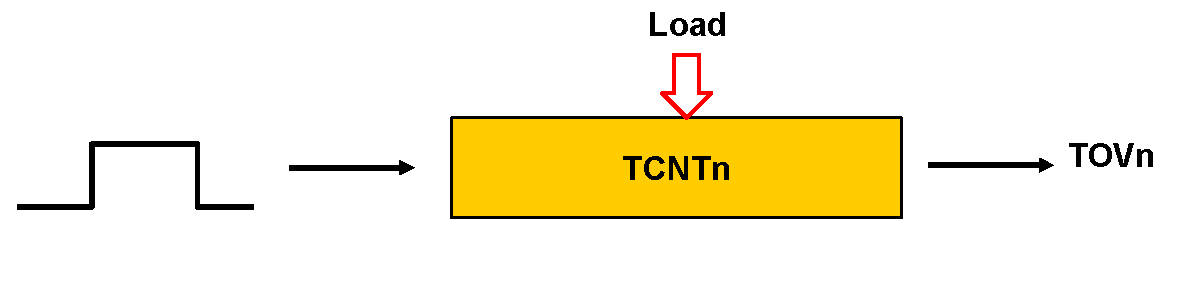
\includegraphics[width = \textwidth]{Graphics/MICROS/Practice 4/SLIDES/OVERFLOW.pdf}
    \caption{Overflow-generated Event~\autocite{SLIDES_MICROS}}
    \label{fig:OVERFLOW}
\end{figure}

\textbf{TCNTn} can be pre-loaded with a value between 0 and maximum value so that the TOVn flag is generated at different time intervals.

\clearpage

\medskip
\underline{\textbf{Match by comparison}}
\medskip

The \textbf{OCRn }register (\textbf{Output Compare Register}) can be loaded with a value between 0 and its maximum value. \textbf{OCRn} and \textbf{TCNTn} are compared in each clock cycle, and a match produces the event, which is indicated by the \textbf{OCFn} (\textbf{Output Compare Flag}) flag.


\begin{figure}[H]
    \centering
    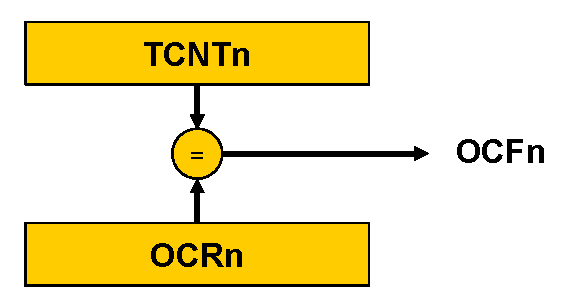
\includegraphics[scale = 0.75]{Graphics/MICROS/Practice 4/SLIDES/COMP_MATCH.pdf}
    \caption{Compare Match-generated Event~\autocite{SLIDES_MICROS}}
    \label{fig:COMPARE_MATCH}
\end{figure}

The resource can be configured so that the timer restarts after a match (\textbf{CTC} mode, \textbf{Clear Timer on Compare Match}).\medskip

In the ATMega328P there are two comparison registers for each timer. Because of that, 6 events can be generated and an automatic response can occur in 6 dedicated terminals.


\medskip
\underline{\textbf{Input capture}}
\medskip

With Timer\_1 it is possible to capture the current value of the timer before external events. A change in the \textbf{ICP1} terminal causes the \textbf{TCT1} record to be read and stored in the \textbf{ICR1} (\textbf{Input Capture Register 1}).

\begin{figure}[H]
    \centering
    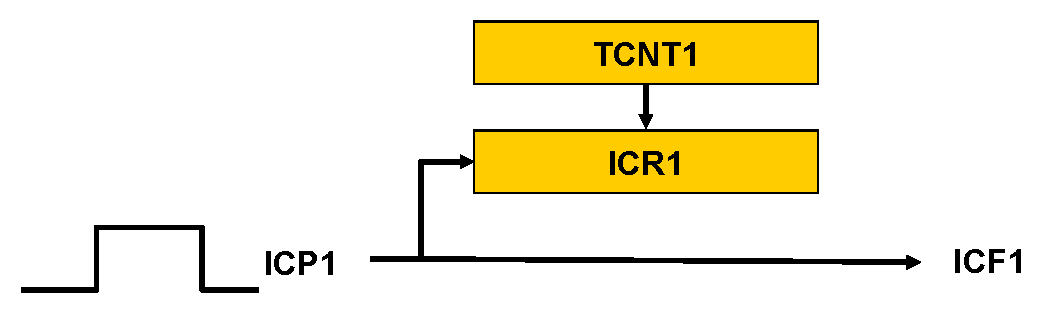
\includegraphics[width = \textwidth]{Graphics/MICROS/Practice 4/SLIDES/INPUT_CAPT.pdf}
    \caption{Input Capture-generated Event~\autocite{SLIDES_MICROS}}
    \label{fig:INPUT_CAPTURE}
\end{figure}

The event is indicated by the ICFn (Input Capture Flag) flag. Since it can be configured to generate an interruption with the rising edge of descent, the events can be useful to measure the width of external pulses.

\clearpage

\paragraph{Prescaler}

A \textbf{prescaler} is an electronic counting circuit used to reduce a high frequency electrical signal to a lower frequency by integer division. The prescaler takes the basic timer clock frequency (which may be the microcontroller clock frequency or may be some higher or lower frequency) and divides it by some value before feeding it to the timer, according to how the prescaler registers are configured.\medskip

In the ATMega328P, Timer\_0 and Timer\_1 share a prescaler, though with independent selection of the divider. Timer\_2, on the other hand, has its own prescaler, with the possibility of being controlled by an external oscillator.\medskip

A diagram showing their internal structure can be seen below:

\begin{figure}[H]
    \centering
    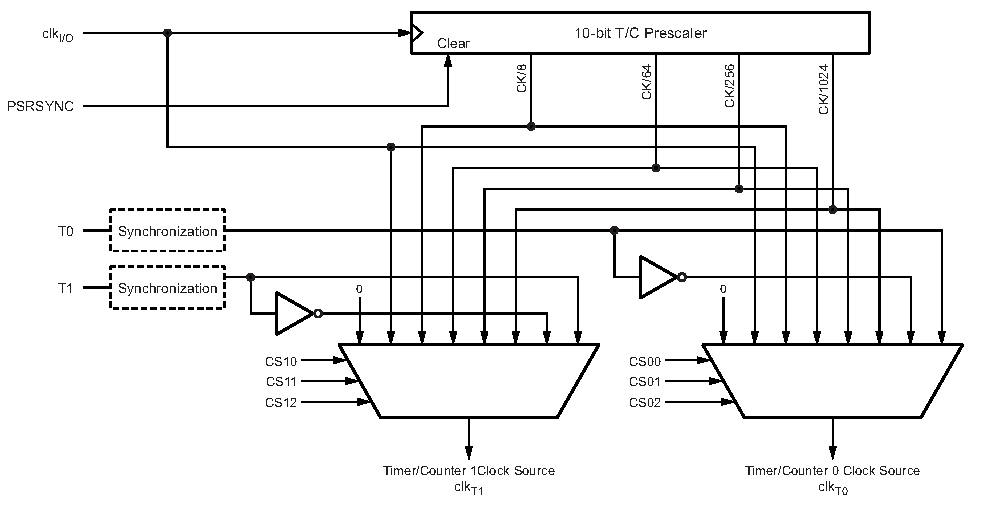
\includegraphics[width = 0.9\textwidth]{Graphics/MICROS/Practice 4/DATASHEET/TIMER10.pdf}
    \caption{Timer\_0 and Timer\_1 Internal Structure}
    \label{fig:TIMER10_PRESCALER}
\end{figure}

\begin{figure}[H]
    \centering
    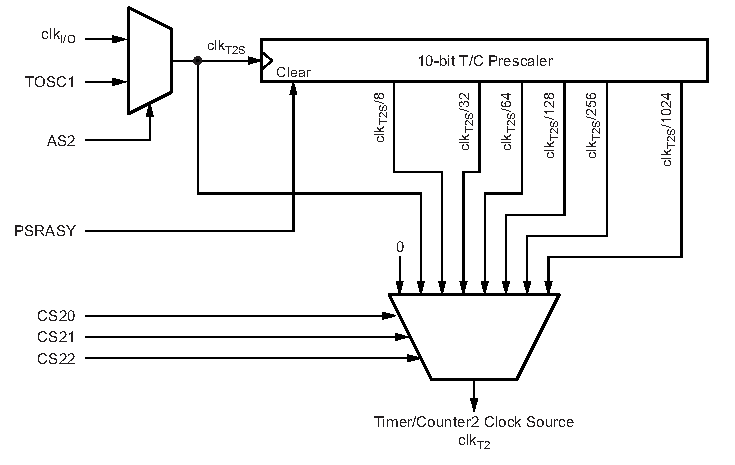
\includegraphics[width = 0.9\textwidth]{Graphics/MICROS/Practice 4/DATASHEET/TIMER2.pdf}
    \caption{Timer\_2 Internal Structure}
    \label{fig:TIMER2_PRESCALER}
\end{figure}


\paragraph{Configuration of timers}

In the case of Timer\_0, is controlled by the following registers:

\medskip
\underline{\textbf{TCCR0A}}
\medskip


\begin{figure}[H]
    \centering
    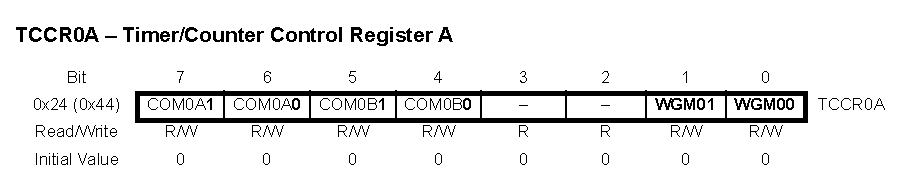
\includegraphics[width = \textwidth]{Graphics/MICROS/Practice 4/DATASHEET/TCCR0A.pdf}
    \caption{Timer/Counter Control Register A}
    \label{fig:TCCR0A}
\end{figure}

There are 6 important bits that must be configured to ensure a proper operation of the timers, namely:

\begin{itemize}
    \item \textbf{Bits [7:6] – COM0A[1:0]: Compare Match Output A Mode} $\bm{\rightarrow}$ These bits control the output compare pin (\textbf{OC0A}) behavior. If one or both of the \textbf{COM0A[1:0]} bits are set, the OC0A output overrides the normal port functionality of the I/O pin it is connected to. However, note that the data direction register (DDR) bit corresponding to the \textbf{OC0A} pin must be set in order to enable the output driver. When \textbf{OC0A} is connected to the pin, the function of the COM0A1:0 bits depends on the WGM02:0 bit setting
    

    \begin{table}[H]
        \resizebox{\columnwidth}{!}{
        \centering
        \begin{tabular}[t]{lccc}
            \toprule
            & \textbf{COM0A1} & \textbf{COM0A0} & \textbf{Description} \\
            \midrule
            & 0 & 0 & Normal port operation, OC0A disconnected.                              \\
            & 0 & 1 & Toggle OC0A on compare match (WGM02 = 1. Normal port operation if 0)   \\
            & 1 & 0 & Clear OC0A on compare match, set OCOA at bottom (Non-Inverting Mode)   \\
            & 1 & 1 & Set OC0A on compare match, clear OCOA at bottom (Inverting Mode)       \\
            \bottomrule
        \end{tabular}
        \caption{Compare Output Mode~\autocite{ATMEGA328P}}
        \label{table:COM0Ax}
        }
    \end{table}


    \item \textbf{Bits [5:4] – COM0B[1:0]: Compare Match Output B Mode} $\bm{\rightarrow}$ Exact same thing as Bits [7:6] but for \textbf{OC0A}
    
    \clearpage

    \item \textbf{Bits [1:0] – WGM0[1:0]: Waveform Generation Mode} $\bm{\rightarrow}$ Combined with the WGM02 bit found in the TCCR0B register, these bits control the counting sequence of the counter, the source for maximum (TOP) counter value, and what type of waveform generation to be used.
    
    \begin{table}[H]
        \resizebox{\columnwidth}{!}{
            \centering
            \begin{tabular}[t]{lcccccccc}
                \toprule
                & \textbf{Mode} & \textbf{WGM02} & \textbf{WGM01} & \textbf{WGM00} & \textbf{Mode of Operation} & \textbf{TOP} & \textbf{Update of OCRx at} & \textbf{TOV Flag Set on}\\
                \midrule

                & 0 & 0 & 0 & 0 & Normal              & 0xFF & Immediate & MAX     \\
                & 1 & 0 & 0 & 1 & PWM, phase correct  & 0xFF & TOP       & BOTTOM  \\
                & 2 & 0 & 1 & 0 & CTC                 & OCRA & Immediate & MAX     \\
                & 3 & 0 & 1 & 1 & Fast PWM            & 0xFF & BOTTOM    & MAX     \\
                & 4 & 1 & 0 & 0 & Reserved            &  -   &  -        &  -      \\
                & 5 & 1 & 0 & 1 & PWM, phase correct  & OCRA & TOP       & BOTTOM  \\
                & 6 & 1 & 1 & 0 & Reserved            &  -   &  -        &  -      \\
                & 7 & 1 & 1 & 1 & Fast PWM            & OCRA & BOTTOM    & TOP     \\
    
                \bottomrule
            \end{tabular}
            \caption{Waveform Generation Mode Bit Description~\autocite{ATMEGA328P}}
            \label{table:WGM0x}
            }
    \end{table}
\end{itemize}



\medskip
\underline{\textbf{TCCR0B}}
\medskip


\begin{figure}[H]
    \centering
    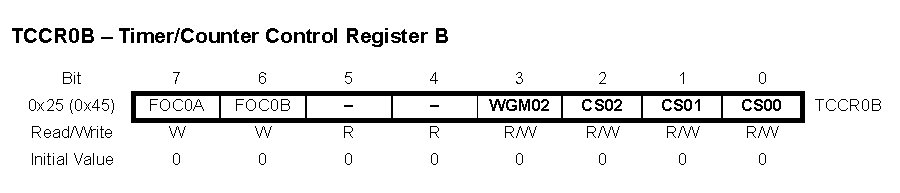
\includegraphics[width = \textwidth]{Graphics/MICROS/Practice 4/DATASHEET/TCCR0B.pdf}
    \caption{Timer/Counter Control Register B}
    \label{fig:TCCR0B}
\end{figure}

There are 6 important bits that must be configured to ensure a proper operation of the timers, namely:

\begin{itemize}
    \item \textbf{Bit [7:6] FOC0A/B: Force Output Compare A/B} $\bm{\rightarrow}$  Force a comparison event, if an automatic response was configured, it will also be performed. FOC0A is related to the OCR0A and FOC0B records with the OCR0B record.
    
    \item \textbf{Bits [2:0] – CS0[2:0]: Clock Select} $\bm{\rightarrow}$ The three clock select bits select the clock source to be used by the Timer/Counter.
    
    \begin{table}[H]
        \resizebox{\columnwidth}{!}{
        \centering
        \begin{tabular}[t]{lcccc}
            \toprule
            & \textbf{CS02} & \textbf{CS01} & \textbf{CS00} & \textbf{Description} \\
            \midrule
            & 0 & 0 & 0 & No clock source (Timer/Counter stopped)                  \\
            & 0 & 0 & 1 & $clk_{I/O}$/(no prescaling)                              \\
            & 0 & 1 & 0 & $clk_{I/O}$/8 (from prescaler)                           \\
            & 0 & 1 & 1 & $clk_{I/O}$/64 (from prescaler)                          \\
            & 1 & 0 & 0 & $clk_{I/O}$/256 (from prescaler)                         \\
            & 1 & 0 & 1 & $clk_{I/O}$/1024 (from prescaler)                        \\
            & 1 & 1 & 0 & External clock source on T0 pin. Clock on falling edge.  \\
            & 1 & 1 & 1 & External clock source on T0 pin. Clock on rising edge.   \\
            \bottomrule
        \end{tabular}
        \caption{Clock Select Bit Description~\autocite{ATMEGA328P}}
        \label{table:CS0x}
        }
    \end{table}
    
\end{itemize}

The events are reflected in the \textbf{TIFR0} (\textbf{Timer/Counter Interrupt Flag Register})

\begin{figure}[H]
    \centering
    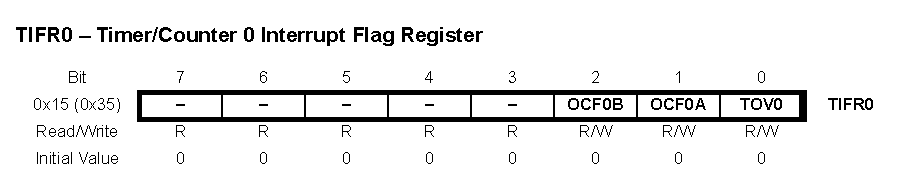
\includegraphics[width = \textwidth]{Graphics/MICROS/Practice 4/DATASHEET/TIFR0.pdf}
    \caption{Timer/Counter 0 Interrupt Flag Register}
    \label{fig:TIFR0}
\end{figure}


There are 3 important bits that must be configured to ensure a proper operation of the timers, namely:

\begin{itemize}
    \item \textbf{Bit [2:1] – OCF0B/A: Timer/Counter 0 Output Compare B/A Match Flag} $\bm{\rightarrow}$ The OCF0B/A bit is set when a compare match occurs between the Timer/Counter and the data in OCR0B/A – output compare register0 B/A. OCF0B/A is cleared by hardware when executing the corresponding interrupt handling vector. Alternatively, OCF0B/A is cleared by writing a logic one to the flag. When the I-bit in SREG, OCIE0B/A (Timer/Counter compare B/A match interrupt enable), and OCF0B/A are set, the Timer/Counter compare match interrupt is executed.
    
    \item \textbf{Bit 0 – TOV0: Timer/Counter0 Overflow Flag} $\bm{\rightarrow}$ The bit TOV0 is set when an overflow occurs in Timer/Counter0. TOV0 is cleared by hardware when executing the corresponding interrupt handling vector. Alternatively, TOV0 is cleared by writing a logic one to the flag. When the
    SREG I-bit, TOIE0 (Timer/Counter0 overflow interrupt enable), and TOV0 are set, the Timer/Counter0 overflow interrupt is executed.
\end{itemize}


In order for the timer/counter\_0 events to produce \textbf{interruptions}, in addition to the Global Enable Bit (bit I in SREG), the interrupts must be activated in the \textbf{TIMSK0} (\textbf{Timer/Counter Interrupt Mask Register 0}).\medskip

The individual enablers are:

\begin{figure}[H]
    \centering
    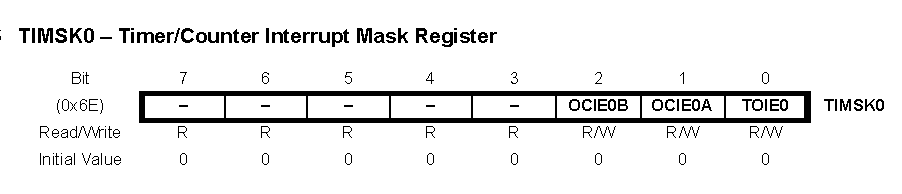
\includegraphics[width = \textwidth]{Graphics/MICROS/Practice 4/DATASHEET/TIMSK0.pdf}
    \caption{Timer/Counter Interrupt Mask Register}
    \label{fig:TIMSK0}
\end{figure}

\clearpage

There are 3 important bits that must be configured to ensure a proper operation of the timers, namely:

\begin{itemize}
    \item \textbf{Bit [2:1] – OCIE0B/A: Timer/Counter Output Compare Match B/A Interrupt Enable} $\bm{\rightarrow}$ When the OCIE0B/A bit is written to one, and the I-bit in the status register is set, the Timer/Counter compare match B/A interrupt is enabled. The corresponding interrupt is executed if a compare match in Timer/Counter occurs, i.e., when the OCF0B/A bit is set in the Timer/Counter interrupt flag register – TIFR0.
    
    \item \textbf{Bit 0 – TOIE0: Timer/Counter0 Overflow Interrupt Enable} $\bm{\rightarrow}$ When the TOIE0 bit is written to one, and the I-bit in the status register is set, the Timer/Counter0 overflow interrupt is enabled. The corresponding interrupt is executed if an overflow in Timer/Counter0 occurs, i.e., when the TOV0 bit is set in the Timer/Counter 0 interrupt flag register – TIFR0.
\end{itemize}

\paragraph{PWM: Pulse-Width Modulation}

Pulse-width modulation (PWM) is a digital technique for varying the amount of power delivered to an
electronic component. The basis of PWM is the variation of the useful cycle (Duty Cycle) of a square signal.\medskip

Changing the duty cycle modifies the average voltage ($V_{AVG}$).

\begin{equation*}
    V_{AVG} = \frac{1}{T} \int_0^{T_{ON}}{V_{PK}\cdot dt\,\,=\,\,V_{PK}\cdot \left( \frac{T_{ON}}{T} \right)}
\end{equation*}

PWM is used in the industry to control devices such as motors, switching power supplies, voltage converters, to name a few.

AVR microcontrollers can handle three types of PWM:

\begin{itemize}
    \item Fast PWM.
    \item Phase Correct PWM.
    \item Phase and Frequency Correct PWM.
\end{itemize}

PWM signals are generated with the operating modes of the timers, in their respective terminals OCxA or OCxB. The modes for the different timers are:

\begin{table}[H]
    \resizebox{\columnwidth}{!}{
    \centering
    \begin{tabular}[t]{lcccc}
        \toprule
        & \textbf{Timer} & \textbf{Fast PWM} & \textbf{Phase Correct PWM} & \textbf{Phase Correct and Frequency Correct PWM} \\
        \midrule
        & 0 & X & X & - \\
        & 1 & X & X & X \\
        & 1 & X & X & - \\
        \bottomrule
    \end{tabular}
    \caption{Timer Modes~\autocite{ATMEGA328P}}
    \label{table:TIMER_MODES}
    }
\end{table}

\clearpage

In this session we will only cover Fast PWM, as it is the most used one and also the easiest to implement.

\medskip
\underline{\textbf{Fast PWM}}
\medskip

Fast PWM allows for higher frequency PWM signals. In this mode the timer counts to its maximum value an then it restarts itself. When a match occurs by comparison, the OCx output goes low, and when the counter reaches its maximum, OCx goes high.\medskip

The PWM frequency for the output can be calculated by the following equation:

\begin{equation*}
    f_{PWM} = \dfrac{f_{CLK}}{N \cdot \mathit{Value}}
\end{equation*}\medskip

\noindent Where \textbf{\textit{N}} is the prescaler, and \textbf{\textit{Value}} is either 256 or OCR0x+1, depending on the TOP value configured on the \textbf{TCCR0A} register. Normally, it is set to 256.\medskip

To enable Fast PWM we must resort back to \textbf{Table \ref{table:COM0Ax}} and \textbf{Table \ref{table:WGM0x}} and configure the corresponding bits. 


\clearpage

\subsection{Exercise 1: Servomotor Control}

Now that all of the necessary concepts have been explained, we will move on to solving the laboratory session itself. \medskip

As we said at the begining of the session, the angle of a servomotor is controlled by connecting its \textit{SIG} terminal to a PWM signal. By changing the duty cycle of the PWM signal we not only change its average value, but also modify the position of the motor's shaft. The duration of the pulse, which has to do with its duty cycle, is standarized. In the image attached below, this behaviour can be observed:

\begin{figure}[H]
    \centering
    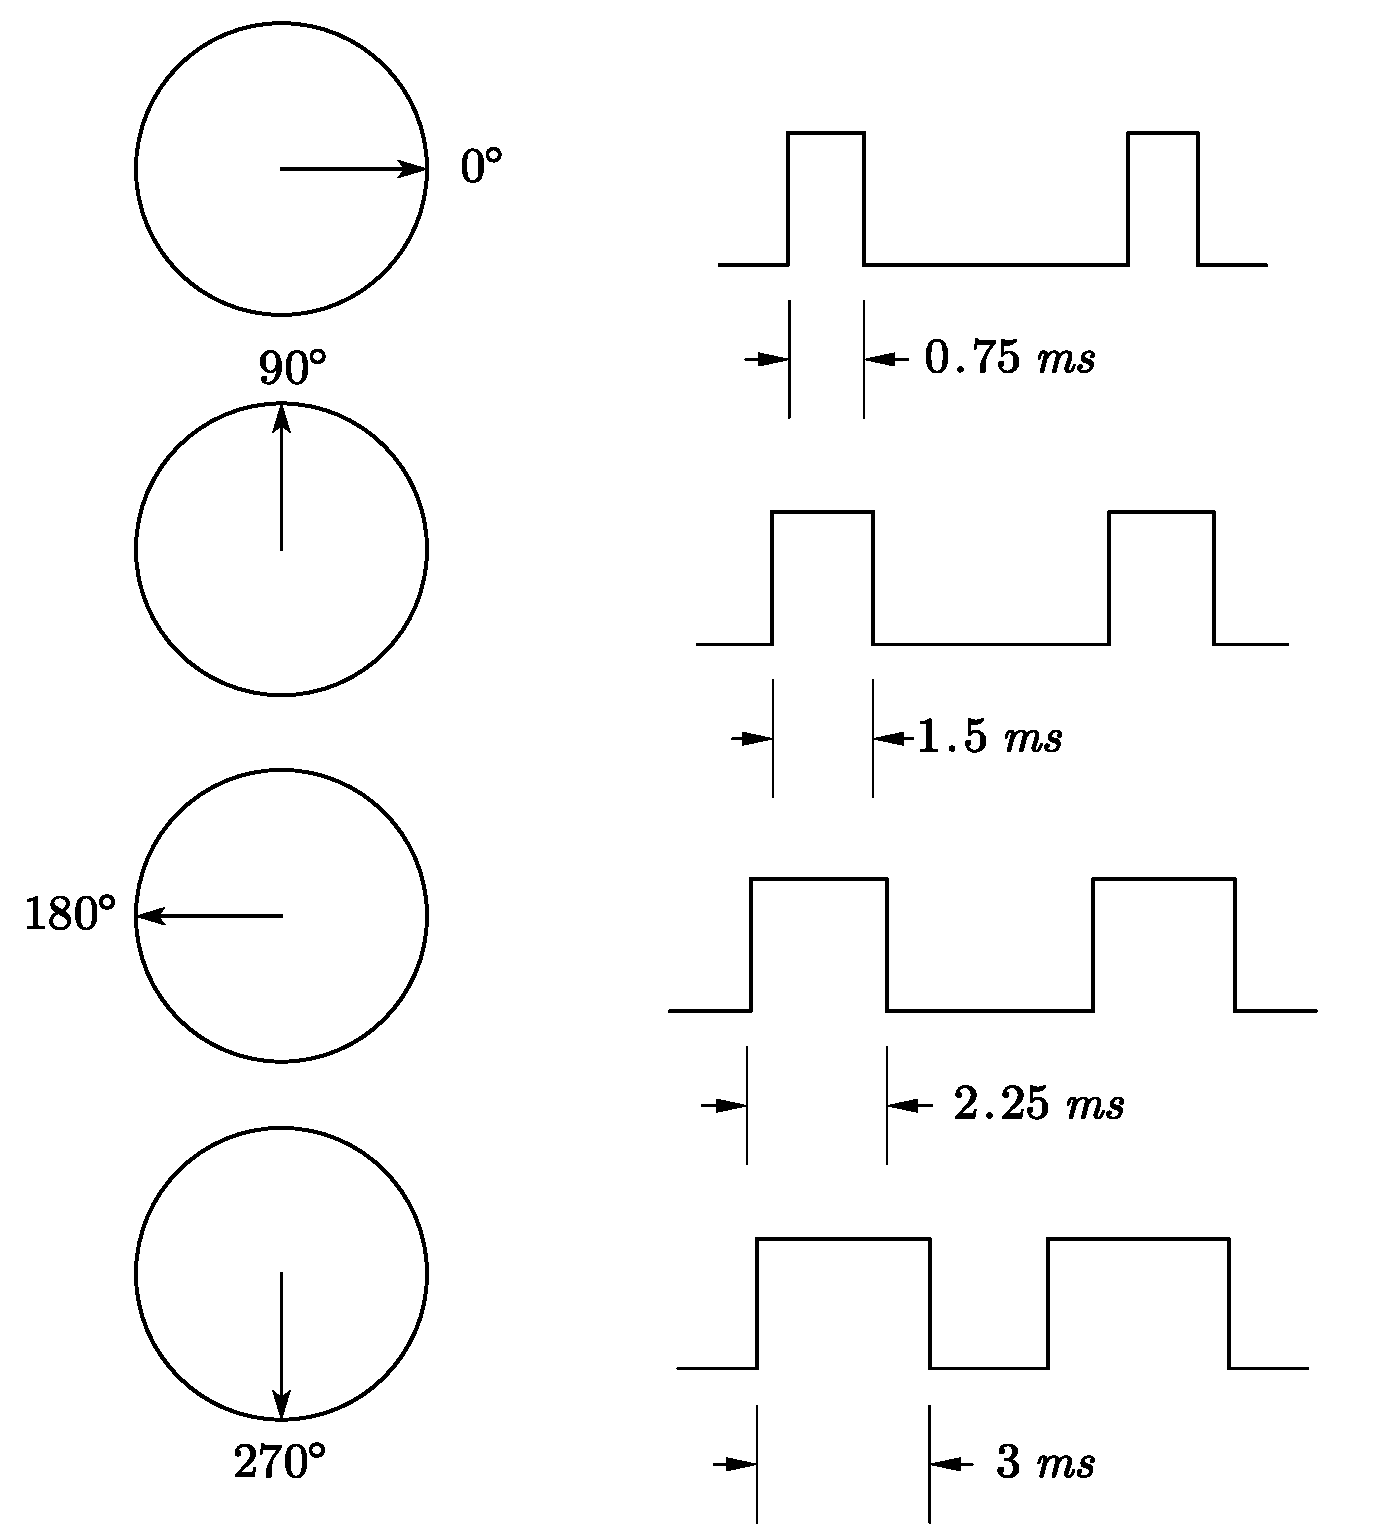
\includegraphics[scale = 0.3]{Graphics/MICROS/Practice 4/SERVO_POSITION.pdf}
    \caption{Servomotor Pulse vs. Angle}
    \label{fig:SERVO_ROTATION}
\end{figure}

It is worth to bear in mind that the maximum angle of rotation of most servomotors is fixed at 180º, though there are some that do not have this limitations.\medskip

The pulse width of the signal will be controlled with the \textbf{Timer 0} of the ATMega328P microcontroller. This timer is nothing but a counter that increases automatically in each instruction cycle or when an external event occurs. \medskip

To set the the amount of time required for a certain pulse width, the \textbf{OCR0A} (\textbf{Output Compare Register A} of the Timer 0) will be used. The \textbf{OCR0A} is an 8-bit register, meaning that it can be set to any value in the range [0:255]. If it is active, whenever the \textbf{TCNT0}, i.e., the value of the timer, reaches the preset value of the \textbf{OCR0A}, the \textbf{OCF0} flag will be set to 1. If the \textbf{CTC (Clear on compare match)} mode is active as well, the timer will restart after a match. This, along with some extra register configurations, can be used to generate a PWM signal.\medskip

Setting a certain value for the \textbf{OCR0A}, and configuring the required registers correctly, will output a signal with a controllable pulse width and therefore, a certain angular position of the servomotor will be obtained.\medskip

In our case, to make the servomotor work properly, the signal that we must obtain will be of the following type: \medskip

\begin{figure}[H]
    \centering
    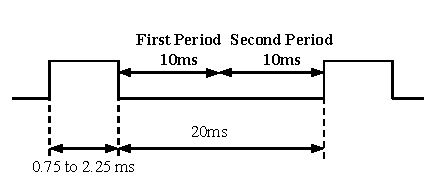
\includegraphics[scale = 1.1]{Graphics/MICROS/Practice 4/SERVO_TIMING.pdf}
    \caption{Needed PWM signal}
    \label{fig:PWM_NEEDED}
\end{figure}


In order to get greater values of the output pulse width than the ones that the 16 MHz clock can provide, the \textbf{prescaler}, which can be configured by modifying the CS0[2:0] bits in the \textbf{TCCR0B} register, is introduced. Its value can be set to 1, 8, 64, 256 and 1024. If the prescaler is set to 8, for example, instead of the counting 1 on each clock cycle, the timer will wait 8 clock cycles to add 1 to the count, i.e. it will slow the counter by a factor of 8.\medskip

As we have seen, the frequency of a \textbf{Fast PWM} signal can be obtained with the following equation:

\begin{equation*}
    f_{PWM} = \dfrac{f_{CLK}}{N \cdot \mathit{Value}}
\end{equation*}\medskip

\noindent Where \textbf{\textit{N}} is the prescaler, and \textbf{\textit{Value}} is either 256 or OCR0x+1, depending on the TOP value configured on the \textbf{TCCR0A} register. Normally, it is set to 256. \medskip

\clearpage

\noindent From this equation we can obtain the value of the prescaler by rearranging the terms.

\begin{equation*}
    N = \dfrac{f_{CLK}}{f_{PWM} \cdot 256}
\end{equation*}\medskip

\noindent From Figure \ref{fig:PWM_NEEDED}, we obtain 3 possible prescalers:

\begin{align*}
    N_{1} &= \dfrac{16 \; MHz}{ \left( \dfrac{1}{0.75 \; ms}\right) \cdot 256} = 47  \\[10pt]
    N_{2} &= \dfrac{16 \; MHz}{ \left( \dfrac{1}{2.25 \; ms}\right) \cdot 256} = 141 \\[10pt]
    N_{3} &= \dfrac{16 \; MHz}{ \left( \dfrac{1}{10 \; ms}\right) \cdot 256} = 625
\end{align*}

For the $T_{ON}$, a prescaler of 256 will be chosen, as it will give a more precise timing. On the other hand, for the $T_{OFF}$, a prescaler of 1024 will be chosen, as there is no other option.\medskip

Two diffenent 10 ms periods have been chosen instead of only one 20 ms period since the maximum $T_{ON}$ allowed by the ATMega328P is around 16 ms.\medskip

To calculate the \textbf{ORCR0A} value needed to obtain the required timing, we will use the following equation:

\begin{equation*}
    \mathbf{OCR0A} = \left( \left(\dfrac{Clock\;freq}{Prescaler}\right) \cdot  T_{ON} \right) - 1 
\end{equation*}

We obtain two values:

\begin{itemize}
    \item 0.75 ms (0 º) $\rightarrow$ OCR0A = 46
    \item 2.25 ms (180 º) $\rightarrow$ OCR0A = 140
\end{itemize}

With these two values we can calculate the equation of the trendline that will give an OCR0A of 140 when the reading of the ADC is equal to 1023 (5 V), and 46 when the reading is equal to 0 (0 V). The obtained equation can be seen below:

\begin{equation*}
    OCR0A = \left( \dfrac{94}{1023} \right) \cdot ADCW + 46
\end{equation*}

\clearpage

To make the program neater, and overall, more visually appealing, we will use a state machine. The states diagram that will be implemented can be seen below:

\begin{figure}[H]
    \centering
    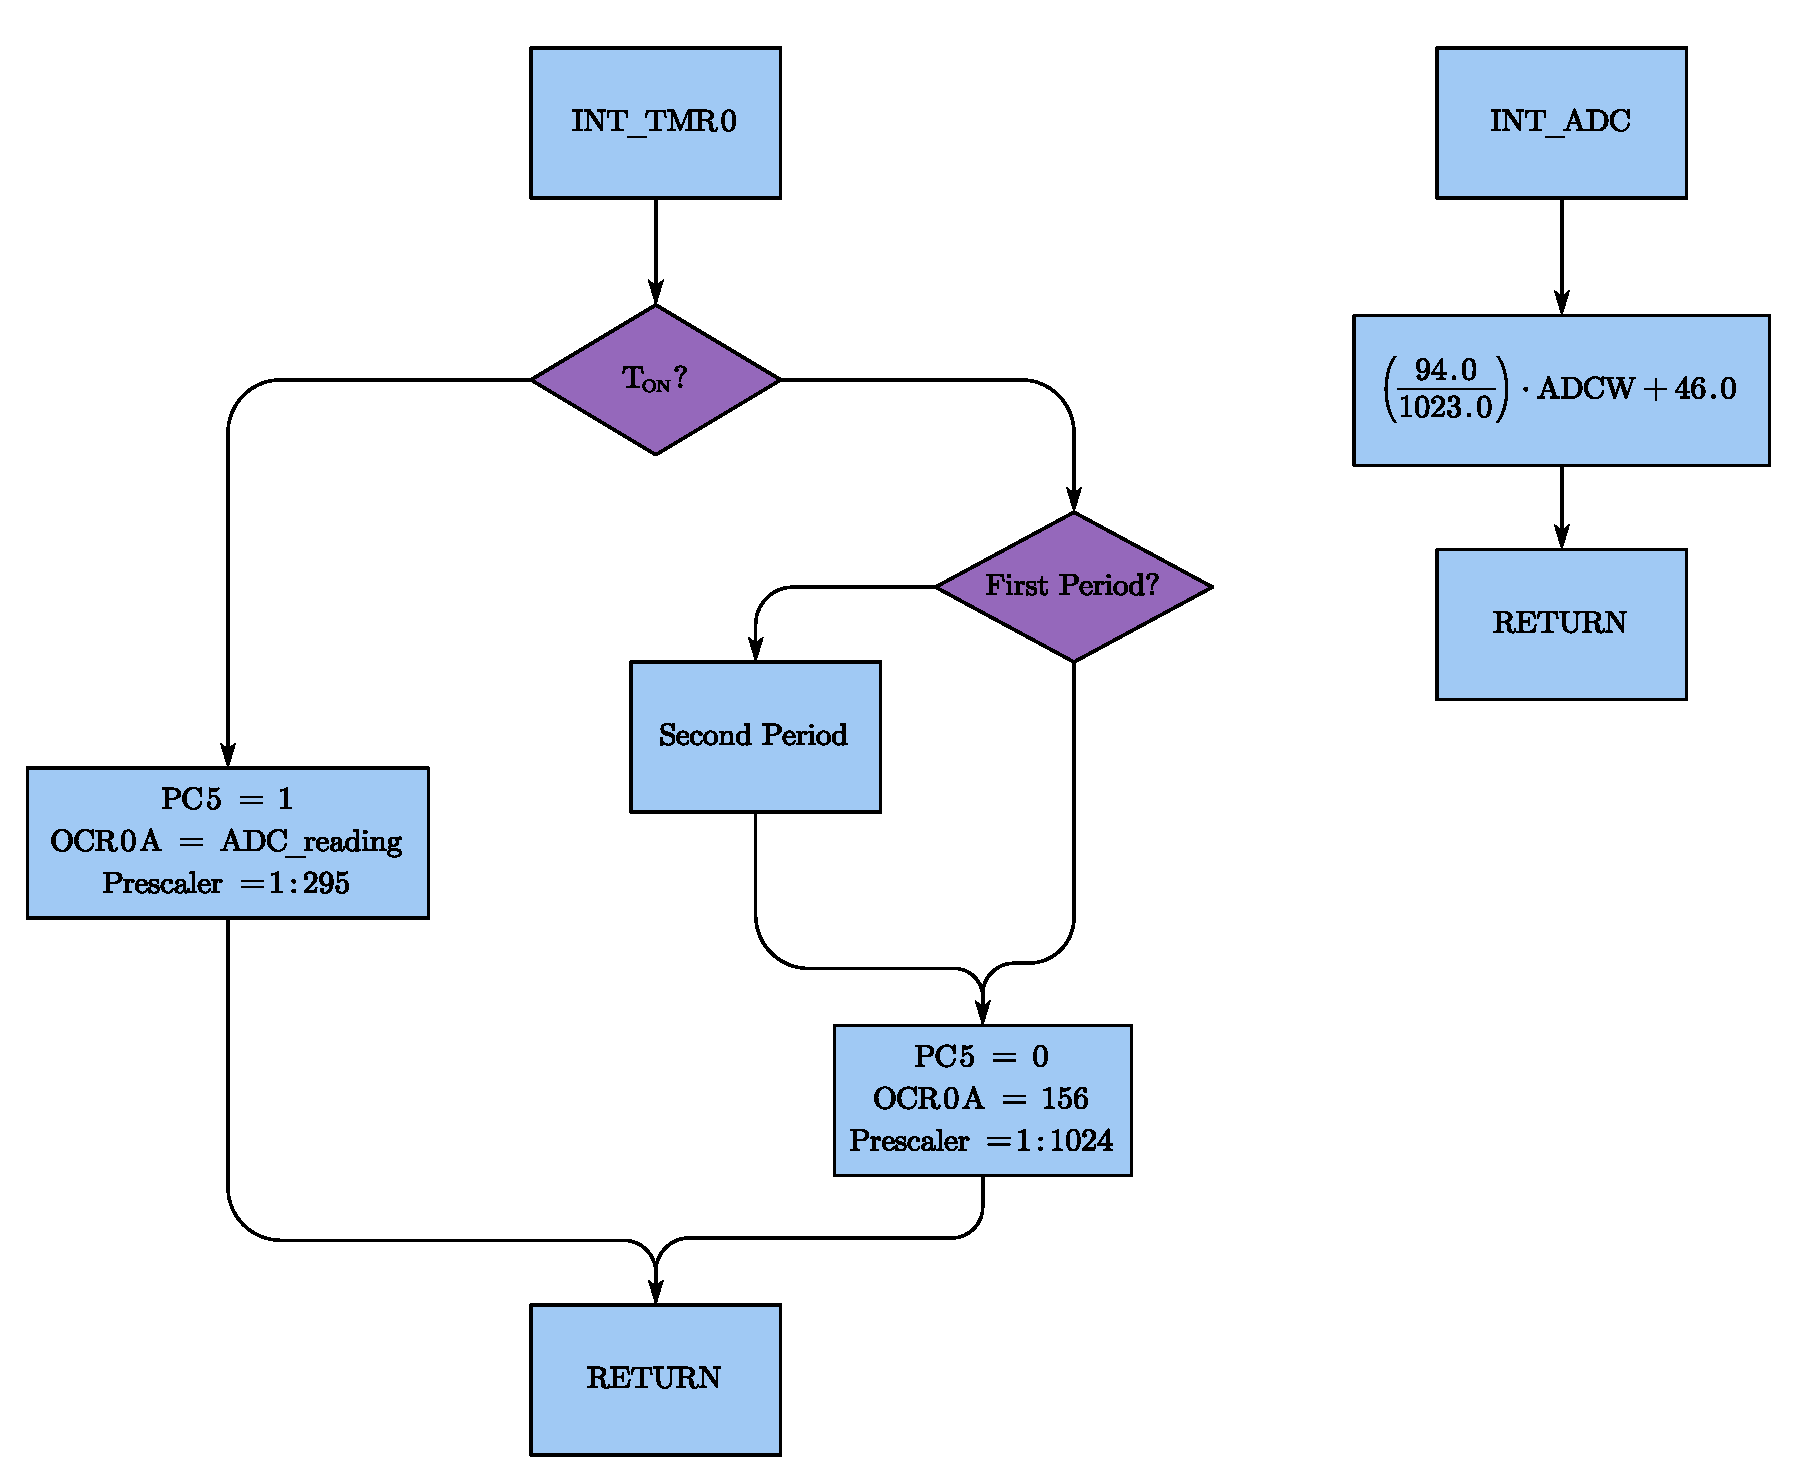
\includegraphics[width = \textwidth]{Graphics/MICROS/Practice 4/STATE_DIAGRAM_TOTAL.pdf}
    \caption{State Diagram and ISRs}
    \label{fig:STATE_DIAG_ISR}
\end{figure}


After calculating all of the needed values and formulas, the proposed code can be finally understood.

\inputCcode{CODES/MICROS/Practice_4/PRACTICE/SERVOMOTOR.c}


After compiling the code, we can simulate it in ISIS Proteus. The following animation shows the angular response of the servo when the input voltage varies from 0 to 5 V:


\begin{figure}[H]
    \centering
 
    \ifnum\value{ANIMATION}=1 {
        \animategraphics[controls,loop,scale=0.85]{1}{Graphics/MICROS/Practice 4/ANIMATION/F}{0}{5}
    } 
    \else {
        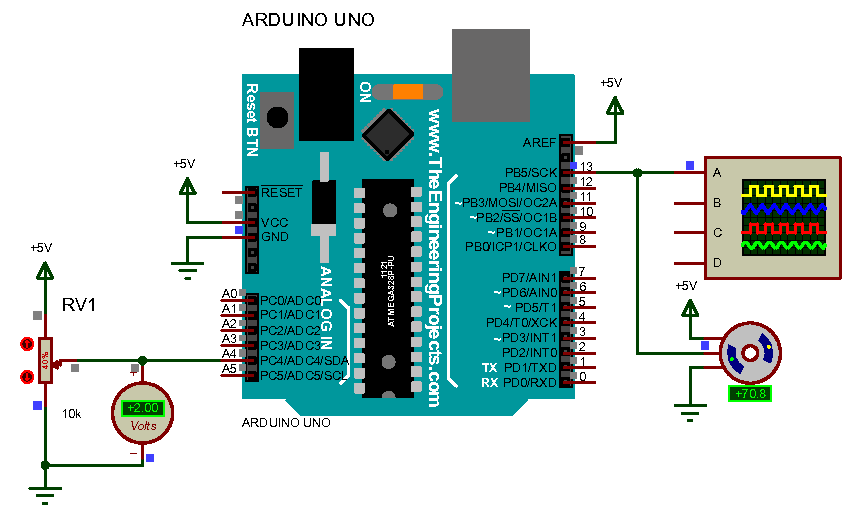
\includegraphics[scale=0.85]{Graphics/MICROS/Practice 4/ANIMATION/F2.pdf}
    }\fi
    
    \caption{Proteus Simulation}
    \label{fig:STEPPER_PROTEUS_MICROS}
\end{figure}




\clearpage





























